% v3批注修改：第一行子图标题与下方线路增加16pt间距，总图题前留7pt。
% 本轮修改：放大相位门圆框和G(θ)门框，保持门中心及连接关系，消除参数文字与边线重叠。
% v2批注修改：原图拆为三个子图；采用Drawio矢量源，浅色门背景、黑色标签；子图标题置底并标红。
\begin{figure*}[!tp]\centering
\begin{minipage}[t]{.48\linewidth}\centering
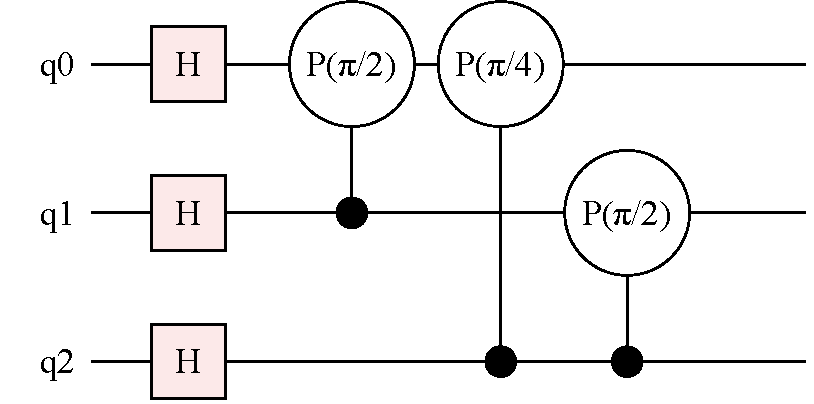
\includegraphics[width=\linewidth,height=32mm,keepaspectratio]{assets/fig10_panel_a_v2.pdf}
\par\vspace{2pt}{\small\color{black}(a) Logical QFT circuit\par}
% 翻译：(a) 逻辑QFT线路。
\end{minipage}\hfill
\begin{minipage}[t]{.48\linewidth}\centering
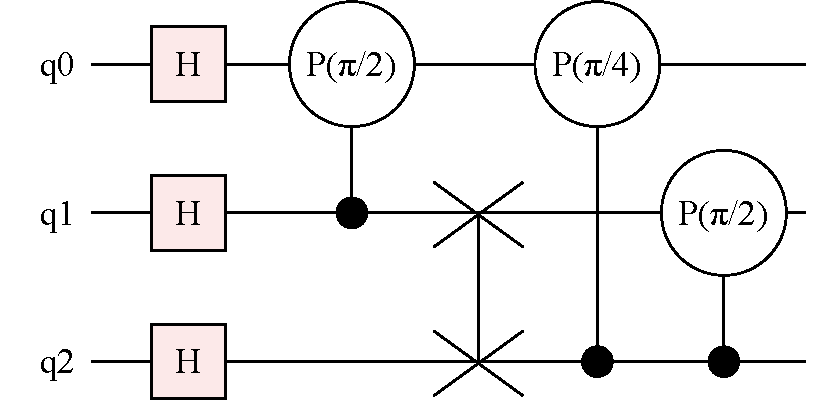
\includegraphics[width=\linewidth,height=32mm,keepaspectratio]{assets/fig10_panel_b_v2.pdf}
\par\vspace{2pt}{\small\color{black}(b) Circuit after topology routing\par}
% 翻译：(b) 拓扑路由后的线路。
\end{minipage}
\par\vspace{16pt}
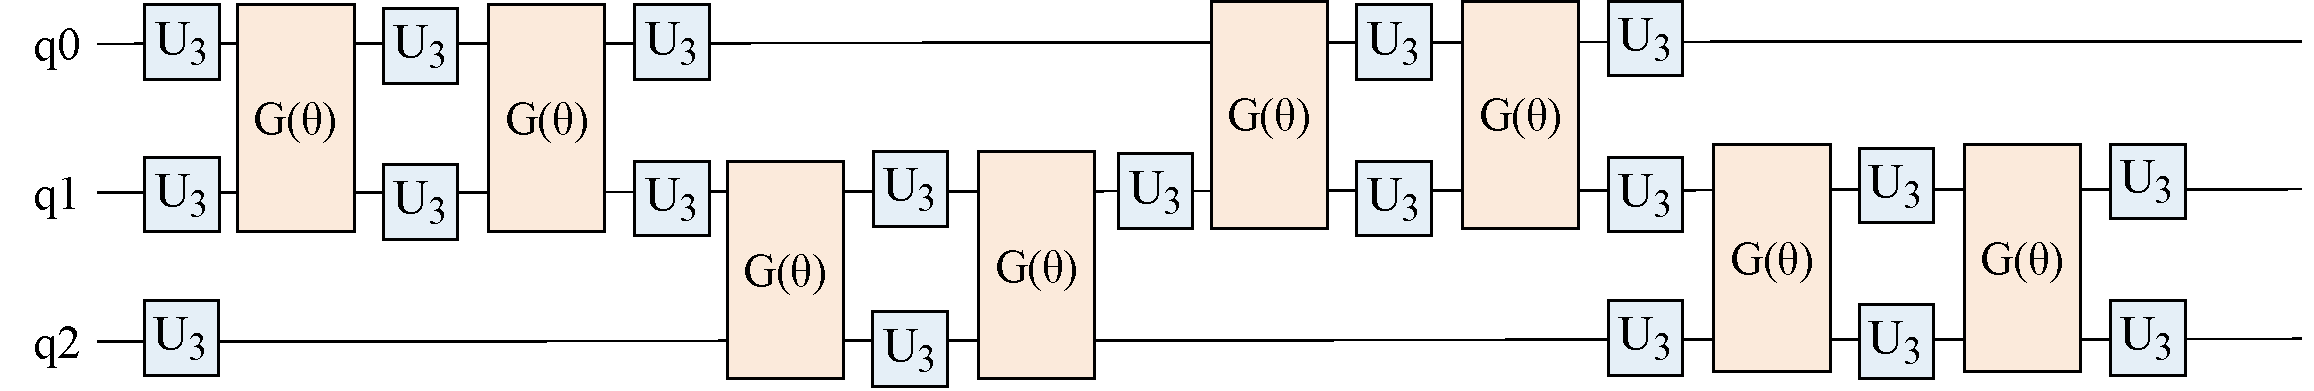
\includegraphics[width=\linewidth]{assets/fig10_panel_c_v2.pdf}
\par\vspace{2pt}{\small\color{black}(c) Executable circuit using $G(\theta)$ and $U_3$\par}
% 翻译：(c) 使用G(θ)与U3的可执行线路。
\par\vspace{7pt}
\caption{Compilation of a QFT circuit with three qubits.}\label{fig:9}
% 翻译：图9：三个量子比特QFT线路的编译过程。
\end{figure*}
